%% This is an example first chapter.  You should put chapter/appendix that you
%% write into a separate file, and add a line \include{yourfilename} to
%% main.tex, where `yourfilename.tex' is the name of the chapter/appendix file.
%% You can process specific files by typing their names in at the 
%% \files=
%% prompt when you run the file main.tex through LaTeX.
\chapter{Continuum Model}

\section{Hyperleastic-Plastic Model} \label{hyperelastic_model}

\section{Hypoelastic-Plastic Model} \label{hypoelastic_model}
In general, hypoelastic models differ from hyperelastic models in that the stress is not obtained from a gradient of a strain energy density function with respect to deformation. The specific hypoelastic granular continuum model used in this study was developed by Dunatunga and Kamrin \cite{Dunatunga:2015:Continuum}. To start one again begins with momentum balance and mass balance
\begin{equation}
\rho\frac{D\bold{v}}{Dt} = \nabla\cdot\bm{\sigma} + \rho\bold{b} \label{mom_bal}
\end{equation}
\begin{equation}
\frac{D\rho}{Dt} + \rho\nabla\cdot\bold{v}=0\label{mass_bal}
\end{equation}
with all terms similarly defined as in the hyperelastic model. A useful quantity, the spatial velocity gradient $\bold{L}$, is defined as
\begin{equation}
\bold{L}=\nabla\bold{v} \label{L_def}
\end{equation}
$\bold{L}$ can be decomposed into a symmetric part (known as the strain rate tensor) and skew part (known as the spin tensor), $\bold{D}$ and $\bold{W}$ respectively, such that
\begin{subequations}
\begin{align}
\bold{L}&=\bold{D}+\bold{W} \label{L_split} \\
\bold{D}&=\frac{1}{2}(\bold{L}-\bold{L}^T) \label{D_def} \\
\bold{W}&=\frac{1}{2}(\bold{L}+\bold{L}^T) \label{W_def}
\end{align}
\end{subequations}
In contrast to the hyperelastic model, the used hypoelastic model takes an additive split of the strain and strain rate-like terms into an elastic and plastic part. For example,
$$\bold{L}=\bold{L}^e+\bold{L}^p$$
The elastic and plastic spatial velocity gradients can then be decomposed into spin and strain rate tensors
$$\bold{L}^e=\bold{D}^e+\bold{W}^e$$
$$\bold{L}^p=\bold{D}^p+\bold{W}^p$$
Due to the fact that a hypoelastic-plastic  model is used and there is no tracking of the deformation gradient, an objective rate must be used to update the stress. While many exist, the Jaumann rate is used here as suggested by Dunatunga and Kamrin, and is defined as
\begin{equation}
\stackrel{\triangle}{\bm{\sigma}}=\dot{\bm{\sigma}}-\bm{W}\cdot\bm{\sigma}+\bm{\sigma}\cdot\bm{W}\label{Jaumann_rate}
\end{equation}
With the basic kinematic variables needed now defined, the next step is defining the constitutive model. As stated in the beginning of this section, this is a hypoelastic-plastic model, and so the elastic constitutive model, plastic yield condition, and plastic flow rule are needed to close the system. The material is assumed to be isotropic and linearly elastic, and the stress is assumed to only be a function of elastic strains. In general the stress rate can then be expressed as a function of the elastic strains contracted with a fourth-order elastic tensor $\mathbb{C}$, or $\stackrel{\triangle}{\bm{\sigma}}=\mathbb{C}:\bm{D}^e$. With the assumptions of isotropocity and first-order linear elasticity, the stress rate can then be more specifically defined as
\begin{equation}
\stackrel{\triangle}{\bm{\sigma}}=2G\bm{D}^e+\lambda tr(\bm{D}^e)\bm{I}\label{constitutive}
\end{equation}
where $G$ is the shear modulus (or second Lam\'e constant) and $\lambda$ is the first Lam\'e constant. However, there is an additional condition on the pressure, which is that
\begin{equation}
	p=
\begin{cases}
	0,							 & \text{if } \rho \leq \rho_c \\
	\frac{K_c}{\rho}(\rho-\rho_c),& \text{if } \rho \geq \rho_c
\end{cases}
\label{pressure_state}
\end{equation}
In other words, if the density of the granular material falls below a certain level, the continuum represents a region of grains that is very loosely packed and has no contacts, and thus cannot support stress. In the physical sense, the grains in this region have entered a gaseous regime (though with no pressure from collisions with the boundary).

The yield condition is very similar in form to a Drucker-Prager yield condition, i.e.
\begin{equation}
\bar{\tau} \leq \mu p \label{yield_condition}
\end{equation}
where $\bar{\tau}$ is the equivalent shear stress and p is the pressure, defined by
\begin{equation}
\bar{\tau}=\sqrt{\frac{1}{2}(\bm{\sigma_0}:\bm{\sigma_0})}\label{tau_bar}
\end{equation}
\begin{equation}
p=-\frac{1}{3}\bm{\sigma}\label{pressure_stress}
\end{equation}
A key difference between the previously explained hyperelastic model and the current hypoelastic model is that the hypoelastic model used by Dunatunga, and subsequently used here, is the introduction of the $\mu(I)$ rheology proposed by Jop et al \cite{Jop:2006:Constitutive}. The $\mu(I)$ rheology proposes a characteristic nondimensional number $I$, defined as
\begin{equation}
I=\dot{\bar{\gamma}}^p\frac{\sqrt{d^2\rho_s}}{\sqrt{p}} \label{inertial_number}
\end{equation}
which gives a measure of the inertia in a sheared granular system relative to the pressure of the system. An empirical fit between $\mu$ and $I$ is given as
\begin{equation}
\begin{cases}
	\mu=\mu(I)=\mu_s+\frac{\mu_2-\mu_s}{I_0/I+1}, & \text{if } I>0 \\
	\mu\leq \mu_s								 & \text{if } I=0
\end{cases}
\label{mu_of_I}
\end{equation}
where $\mu_s$, $\mu_2$ and $I_0$ are material parameters. As suggested by \ref{mu_of_I}, $\mu_s$ is a static friction coefficient, or the value of friction in the limit that $I$ approaches 0. As $I$ approaches infinity $mu$ approaches $mu_2$. Though the existence of an asymptotic $\mu_2$ is still debated in literature, it serves as a good approximation for the levels of $I$ reached in the simulations run in this study. Thus the plastic yield condition utilized here is more exactly stated as
\begin{equation}
\bar{\tau} \leq \mu(I) p \label{yield_condition_mu_of_I}
\end{equation}

At plastic yielding, a flow rule must be defined to evolve the plastic strain. A commonly taken assumption that is also taken here is one of spin-less plastic flow, so that $\bold{W}^p=\bold{0}$ and $\bold{L}^p=\bold{D}^p$. Plastic flow codirectionality with the stress deviator and isochoric plastic flow are also taken as assumptions, leading to an plastic flow rate of
\begin{equation}
\bold{L}^p=\bold{\hat{D}}^p(\bm{\sigma})=\frac{1}{\sqrt{2}}\dot{\bar{\gamma}}^p(\bm{\sigma})\frac{\bm{\sigma}_0}{||\bm{\sigma}_0||}\label{flow_rule}
\end{equation}
where $\dot{\bar{\gamma}}^p$ is the equivalent plastic shear strain rate.

As a final note, there is a desired behavior of a "no tension" rule, in that granular media can not support tensile stress states. While this is partly captured by the pressure dependence on the material density relative to a critical density expressed in \ref{pressure_state}, another check must be done. In the constitutive update to evolve the stress, if it is determined that the pressure of the material is negative (i.e. the material wants to contract in on itself because of volumetric tensile stresses), then the stress is set to 0. Exact implementation details of the stress update can be found in Dunatunga et al, with the relevant density and pressure checks of that update being most relevant for hybridization purposes. 

\section{Material Point Method}
In order to discretize and solve the equations defined in the previous sections, an appropriate method must be chosen. Classically the finite element method has been the method of choice for problems involving solid mechanics. As stated before however, a singular granular system, i.e. flow in an hourglass, has that granular system existing in multiple states at once: a solid bottom pile, a flowing regime down the top of the pile and at the top flowing into the hourglass neck, and a gaseous regime as it exits the neck. Using a method like the finite element to track the deformation of the granular continuum would be nearly impossible, due to the large amounts of non-affine strain that accumulate in the system causing mesh inversions. Remeshing, or a method like the Arbitrary-Lagrangian-Eularian method, could at first glance help resolve this. However the amount of remeshing that needs to occur would incur both a computational penalty for the remeshing algorithm, but also an accuracy penalty due to the need to constantly interpolate quantities.

On the other hand, methods used to solve equations in an Eularian frame for fluid mechanics, like the finite volume method, may then seem appealing. Finite volume however brings with it its own drawbacks in the context of granular media. Finite volume methods have trouble modeling purely solid regimes \textcolor{red}{FINDREFERENCE}. They also do not inherently track free surfaces like Lagrangian finite element would. This free surface tracking is crucial in the problems of interest in granular media study, as the evolution of the free surface, and the interactions of the free surface with surrounding matter, are what ultimately matter in, for example studying the effects of a landslide on anything downhill of the flow zone. Breakaway of granular material from an initial agglomeration of material and the ability to divide that agglomeration into smaller bodies of granular material are also behaviors that are exhibited that cannot be easily captured by finite volume.

The ideal method then is Lagrangian, can track free surfaces, can also handle the large non-affine strains introduced in the liquid and gaseous regimes of granular flow. A class of methods, called particle methods, aim to solve this niche of problem by tracking the evolution of the system through particles, instead of with a mesh. Many types of course exist, including the popular smoothed-particle hydrodynamics (SPH) diffusive element method, and the reproducing kernal method (RKPM) \textcolor{red}{FINDREFERENCE}. All vary in their exact discretization of continuum quantities, representation of connectivity between points, and other details. The continuum discretization method used in this study, known as the Material Point Method (MPM), is a framework that both provides familiarity with methods like the finite element method while adding on the abilities desired.

MPM was developed in the mid 1990s by Sulsky et al and has enjoyed much use and development since \cite{Sulsky:1994}\textcolor{red}{FINDREFERENCE}. MPM is what is known as a mesh-free method, which as the name implies, denotes that there is no permanent mesh used to track deformation. This lack of a permanent mesh of course avoids the mesh deformation issue entirely. As a brief history aside, MPM is a derivative of the fluid-implicit-particle method (FLIP), which is itself a derivative of the particle-in-cell (PIC) method, where PIC was developed in the context of building a method to solve for fluid flow in a Lagrangian frame. Properties of both methods explicitly arise in MPM, which will be discussed later.

\subsection{MPM Algorithm Overview}

\begin{figure}[htp] 
    \centering
    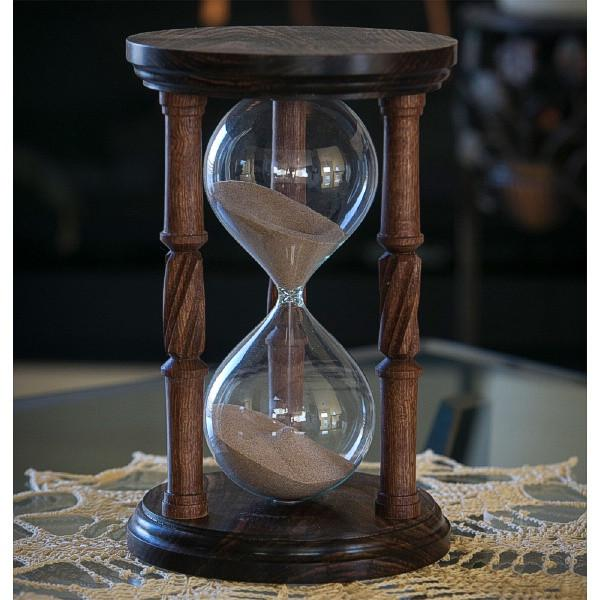
\includegraphics[width=0.4\textwidth]{figs/hourglass_whole.jpg}
    \caption{Schematic of a single timestep in MPM.}
    \label{MPM_diagram}
\end{figure}

In MPM, a continuum body is first discretized via Lagrangian markers, known as MPM points. Quantities of interest, like mass, momentum, stress, and any internal variables, are held on these points. It should be noted that there is no explicit notion of connectivity stored on the points between pairs or groups of points, and so no nearest-neighbor search must be conducted, like in SPH or many other particle methods. A temporary (with an emphasis on the "temporary", as the introduction of a mesh may seem contradictory to MPM being classified a mesh-free method) background grid is then introduced as a "computational scratch-pad" . The aforementioned quantities of interest are then projected onto the background grid with a chosen set of basis functions. As a note, while there is no strict requirement on the discretization of the background grid, often a simple Cartesian grid is chosen for convenience. With these quantities now having a nodal representation on the grid, a finite element-like update is conducted. The updated nodal quantities are then projected back onto the MPM points, so that the points are now in an updated state. The background grid is then destroyed, so that no accumulation of strain occurs. With new point quantities, the points are then advected, completing a timestep of MPM.

\subsection{MPM Formulation and Discretization}
As shown schematically in the previous section, at the beginning of a timestep $n$, each MPM point $p$ has stored on it its position ${\bm{x}_p}^n$, velocity ${\bm{v}_p}^n$, mass ${m_p}^n$, velocity gradient ${\bm{L}_p}^n$, Cauchy stress ${\bm{\sigma}_p}^n$, volume ${V_p}^n$, and for the hyperelastic case, ${{\bm{B}_p}^e}^n$ and ${J_p}^n$. The grid projection of any point quantity $\bm{\phi}_p$ onto a node i is done via the operation
\begin{equation}
\phi_i=\sum_pS_{ip}{\bm{\phi}}_p\label{projection_value}
\end{equation}
where $S_{ip}$ is the value of the basis function $S_i$ at location $\bm{x}_p$, or $S_{ip}=S_i{\bm{x}_p}$. Likewise the grid projection of the gradient of any point quantity $\bm{\phi}_p$ onto a node i is done via the operation
\begin{equation}
\nabla \phi_i=\sum_p \nabla S_{ip}{\bm{\phi}}_p \label{projection_gradient}
\end{equation}
While one is free to choose from any number of function spaces for the basis functions, two types are used in this study. The first are classic linear "hat" functions, which in 1D are defined as
\begin{equation}
S_i(x)=max[0,(1-\frac{|x_i-x|}{h})]\label{linear_basis}
\end{equation}
where h is the element length. The gradient is then defined as
\begin{equation}
	\nabla S_i(x)=
\begin{cases}
	\frac{sgn(x_i-x)}{h},     & \text{if } |x_i-x| \leq h \\
	0,						 & \text{otherwise}
\end{cases}
\label{linear_basis_gradient}
\end{equation}
The second class of basis functions used are known as GIMP (Generalized Interpolation Material Point) basis functions. GIMP basis functions take into account a finite size for the points (instead of a delta function classically used), and integrate the bases across this point domain. This extended support for the GIMP basis functions result in smoother grid crossings and higher order approximations. First order GIMP basis functions (resulting in 2nd order field approximations) were used, with details being found in \cite{Bardenhagen:2004}.

The product of these basis functions in additional directions in 2D and 3D then form the basis in those dimensions.

Note that from now on, all basis function values are taken for the point locations at time $n$, and so for brevity the superscript $n$ is not included for the basis functions $S_{ip}$ and gradients $\nabla S_{ip}$. To begin, the point masses and momenta are projected onto the nodes via the operations previously described. 
\begin{equation}
{m_i}^n=\sum_pS_{ip}{m_p}^n,\ ({{\bm{mv}}_i})^n=\sum_pS_{ip}({{\bm{mv}}_p})^n\label{mass_and_mom_projection}
\end{equation}
For the hypoelastic model, the point volumes and stresses are then updated. The volume update is described by
\begin{equation}
{V_p}^{n+1}={V_p}^n exp(\Delta tr\bm{L}^n) \label{volume_update}
\end{equation}
The stress update is then calculated with the constitutive law described in Section \ref{hypoelastic_model}, and the exact numerical implementation can be found in Dunantunga and Kamrin \cite{Dunatunga:2015:Continuum}. In the hyperelastic case, the volumetric strain $J$ and stress are also updated here, as described in \ref{hyperelastic_model}.
The external forces ${\bm{b}_i}^n$ and internal forces ${\bm{f}_i}^n$ (internal forces being derived from the divergence of the just-calculated Cauchy stress) are then projected to the grid.
\begin{equation}
{\bm{b}_i}^n=\sum_pS_{ip}{m_p}^n{\bm{b}_p}^n,\ {\bm{f}_i}^n=\sum_p -V_p\bm{{\sigma}_p}^n \cdot \nabla S_{ip}
\label{force_projection}
\end{equation}
Now, the nodes contain both the current momentum and current forces. The change in nodal momentum is then given by
\begin{equation}
\dot{(\bm{mv})^n_i}=\sum_{i}\bm{F}^n_i=\bm{b}^n_i+\bm{f}^n_i\label{momentum_rate}
\end{equation}
The time integration of the nodal momentums can then be done a number of ways, but here a simple forward euler is used, which produces
\begin{equation}
(\bm{mv})^{n+1}_i=(\bm{mv})^n_i+\Delta t(\bm{b}^n_i+\bm{f}^n_i)
\end{equation}
Nodal interactions with boundaries are then taken into account. In the current code, two types of boundaries are supported: "sticky" rigid planes and "sliding" rigid planes. The algorithm for this interaction check loops through all grid nodes $i$, and checks to see if any mass has been projected to the node. If so, then the code loops through all defined planes, calculating the distance of the grid point to the given plane, to check for a nodal collision with the plane. If there is a collision found, then the relative velocity of the point to the plane is calculated. For a "sliding" boundary, the normal relative momentum is set to zero (allowing movement in the tangential velocity, and hence the "sliding"), while in the "sticky" boundary case the entire nodal momentum $(\bm{mv})^{n+1}_i$ is set to $\bm{0}$.

Next, the new nodal velocities and accelerations are calculated as
\begin{equation}
\bm{v}^{n+1}_i=(\bm{mv})^{n+1}_i/m^n_i
\end{equation}
\begin{equation}
\bm{a}^{n+1}_i=\frac{(\bm{mv})^{n+1}_i-(\bm{mv})^n_i}{\Delta t m^n_i}
\end{equation}
The new nodal velocities are used to calculate the new velocity gradients $\bm{L}^{n+1}_p$ on the points with
\begin{equation}
\bm{L}^{n+1}_p=\sum_{i}\bm{v}^{n+1}_i \otimes\nabla S_{ip}
\end{equation}
In the hyperlastic model, the elastic prediction and plastic correction steps are then conducted, as explained in \ref{hyperelastic_model}.

The next step, the update of the point velocity, is one that deserves extra attention. Two quantities are temporarily introduced, the PIC velocity $\bm{v}_{pic}$ and the point acceleration $\bm{a}_p$, defined as
\begin{equation}
\bm{v}_{pic}=\sum_{i}S_{ip}\bm{v}^{n+1}_i
\label{pic_update}
\end{equation}
\begin{equation}
\bm{a}_p=\sum_{i}S_{ip}\bm{a}^{n+1}_i
\end{equation}
From this it can be seen that there are two possible avenues to update the point velocity to $\bm{v}^{n+1}_p$. One, called the PIC update (so-called because this is the point velocity update that the PIC method used), directly uses the $\bm{v}_{pic}$ velocity as the new point velocity, so $\bm{v}^{n+1}_p=\bm{v}_{pic}$. This means that the point velocities are directly interpolated from the background grid velocities, and thus the velocity field is constrained by the basis functions. The other, called the FLIP update (again so-called because FLIP uses this as its velocity update), instead uses the nodal accelerations to construct a point acceleration. The FLIP velocity, $\bm{v}_{flip}$ is then obtained by
\begin{equation}
\bm{v}_{flip}=\bm{v}^n_p+\Delta t \bm{a}_p
\label{flip_update}
\end{equation}
With this construction, the velocities live in a higher order vector space, allowing for higher order kinematic modes. The macroscopic result of these two updates is that, often, flows with PIC updates have a high degree of dissipation and do not conserve angular momentum. Physically realistic voritical flow and oscillations either do not appear or are quickly damped. This dissipative quality however means that PIC schemes are often stable. On the other hand, FLIP updated flows more often preserve those vortical effects and oscillations and better conserve angular momentum. This though means that instabilities can form and will not be damped out. 

A strategy that is used to obtain some middle ground between the two strategies is to simply take a linear combination of the two updates. This is expressed functionally as
\begin{equation}
\bm{v}^{n+1}_p=(1-\alpha)\bm{v}_{pic} + \alpha \bm{v}_{flip}
\end{equation}
where $\alpha$ is a parameter used to tune how much one wants a PIC vs a FLIP update. A large $\alpha$ value is often used, as better angular momentum conservation is usually desired over better numerical stability, though a small portion of PIC velocity still helps with stability. In this study, $\alpha$ was set to between 0.95 and 1.0 for all simulations. 

Finally, the points are advected. 

As alluded to with the "FEM-like solve", MPM can be interpreted as a finite element method, with a single point 